\subsection{实验目的-实现外部 IP 地址映射到服务器}
使用 iptables 命令配置防火墙,实现外部 IP 地址映射到服务器.
%
\subsection{实验原理}
通过配置 NAT 表实现外部 IP 地址映射到服务器.
%
\subsection{实验环境}
操作系统:
\begin{itemize}
  \item Windows 7
  \item Windows server 2003
  \item CentOS 6.5
\end{itemize}
%
\subsection{实验步骤}
\subsubsection{将外部 IP 端口地址映射到内部服务器}
打开防火墙 CentOS 6.5 的终端,输入命令
\begin{minted}[bgcolor=bg,breaklines=true]{sh}
lsof -i :80
\end{minted}
若无 http 服务,输入
\begin{minted}[bgcolor=bg,breaklines=true]{sh}
/etc/init.d/httpd start
\end{minted}
开启 http 服务,
再使用
\begin{minted}[bgcolor=bg,breaklines=true]{sh}
lsof -i :80
\end{minted}
进行查看时,可以看到 http 服务已成功开启。
\begin{figure}[H]
  \begin{center}
    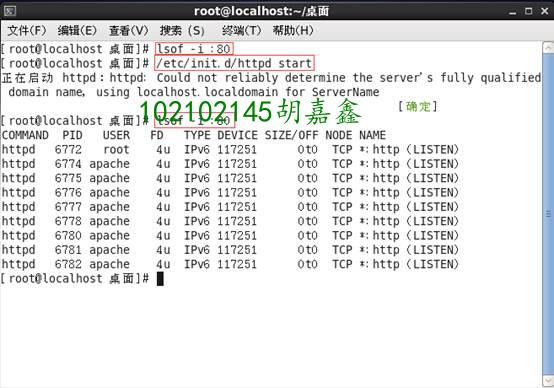
\includegraphics[width=0.40\textwidth]{2_9_1.jpeg}
  \end{center}
\end{figure}

此时防火墙 nat 表无规则。
\begin{figure}[H]
  \begin{center}
    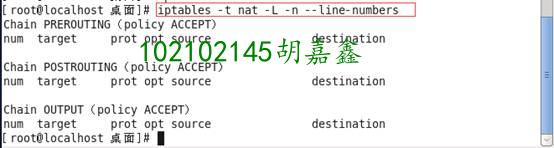
\includegraphics[width=0.40\textwidth]{2_9_2.jpeg}
  \end{center}
\end{figure}

此时在 Windows 7 上打开火狐浏览器,在地址栏输入
\texttt{http://192.168.1.200},打开的是防火墙 CentOS 6.5 上的
http 服务,即 Apache。
\begin{figure}[H]
  \begin{center}
    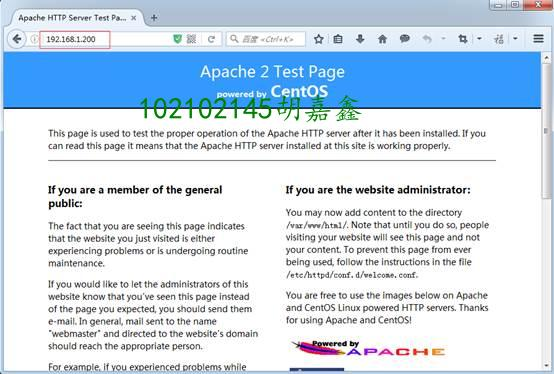
\includegraphics[width=0.40\textwidth]{2_9_3.jpeg}
  \end{center}
\end{figure}

在防火墙 CentOS6.5 的终端输入命令
\begin{minted}[bgcolor=bg,breaklines=true]{sh}
echo 1 > /proc/sys/net/ipv4/ip_forward
\end{minted}
开启防火墙数据包转发功能。
输入命令
\begin{minted}[bgcolor=bg,breaklines=true]{sh}
cat /proc/sys/net/ipv4/ip_forward
\end{minted}
进行查看。
此外,必须保证 \texttt{/etc/sysctl.conf} 文件中
\mintinline{sh}{net.ipv4.ip_forward} 的值为 1。
\begin{figure}[H]
  \begin{center}
    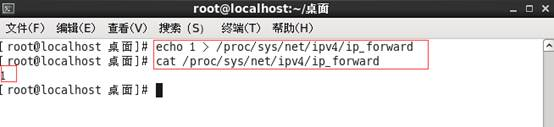
\includegraphics[width=0.40\textwidth]{2_9_4.jpeg}
  \end{center}
\end{figure}
\begin{figure}[H]
  \begin{center}
    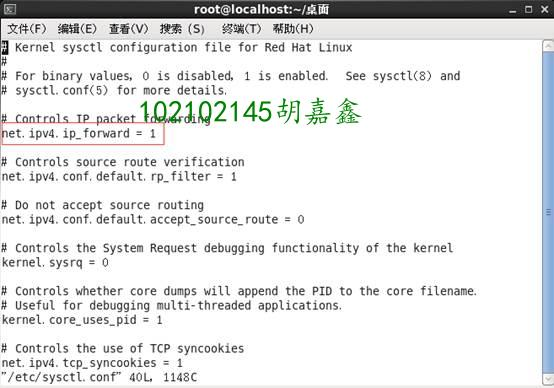
\includegraphics[width=0.40\textwidth]{2_9_5.jpeg}
  \end{center}
\end{figure}

在防火墙 CentOS 6.5 的终端输入如下命令,
\begin{minted}[bgcolor=bg,breaklines=true]{sh}
iptables -t nat -A PREROUTING -d 192.168.1.200 -p tcp --dport 80 -j DNAT --to-destination 20.0.0.2:80
iptables -t nat -A POSTROUTING -d 20.0.0.2 -p tcp --dport 80 -j SNAT --to-source 192.168.1.200
iptables -t nat -L -n --line-numbers
\end{minted}
将外部 IP 地址端口 \texttt{192.168.1.200:80} 映射到内部服务器
\texttt{20.0.0.2:80}。
\begin{figure}[H]
  \begin{center}
    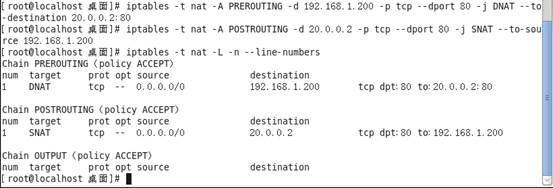
\includegraphics[width=0.40\textwidth]{2_9_6.jpeg}
  \end{center}
\end{figure}

在终端输入命令
\begin{minted}[bgcolor=bg,breaklines=true]{sh}
/etc/init.d/iptables save
\end{minted}
保存配置的防火墙规则。
输入命令
\begin{minted}[bgcolor=bg,breaklines=true]{sh}
cat /etc/sysconfig/iptables
\end{minted}
查看配置的防火墙规则。
\begin{figure}[H]
  \begin{center}
    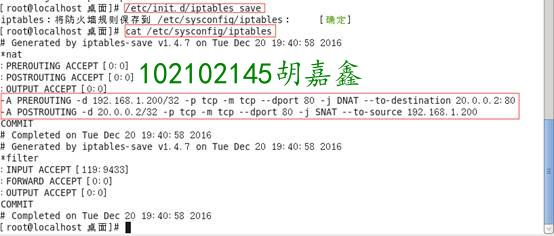
\includegraphics[width=0.40\textwidth]{2_9_7.jpeg}
  \end{center}
\end{figure}

此时在操作机Windows7上访问
\texttt{http://192.168.1.200}时访问的是内部服务器的网站
\texttt{http://20.0.0.2}。
\begin{figure}[H]
  \begin{center}
    
\includegraphics[width=0.40\textwidth]{2_9_8.jpeg}
  \end{center}
\end{figure}
